\chapter{PJ3}

\section{程式}

操控球員程式:
\begin{lstlisting}[language=Python, frame=single, numbers=left, captionpos=b, basicstyle=\ttfamily\small, showstringspaces=false, breaklines=true, tabsize=4, xleftmargin=15pt]
# pip install pyzmq cbor keyboard
from zmqRemoteApi_IPv6 import RemoteAPIClient
import keyboard
 
client = RemoteAPIClient('localhost', 23000)
 
print('Program started')
sim = client.getObject('sim')
 
 
 
sim.startSimulation()
print('Simulation started')
 
def setBubbleRobVelocity(leftWheelVelocity1, rightWheelVelocity1, leftWheelVelocity2, rightWheelVelocity2):
    leftMotor1 = sim.getObject('/81')
    rightMotor1 = sim.getObject('/82')
    leftMotor2 = sim.getObject('/83')
    rightMotor2 = sim.getObject('/84')
    sim.setJointTargetVelocity(leftMotor1, leftWheelVelocity1)
    sim.setJointTargetVelocity(rightMotor1, rightWheelVelocity1)
    sim.setJointTargetVelocity(leftMotor2, leftWheelVelocity2)
    sim.setJointTargetVelocity(rightMotor2, rightWheelVelocity2)
    
 
'''
# Example usage 1:
setBubbleRobVelocity(1.0, 1.0)
time.sleep(2)
setBubbleRobVelocity(0.0, 0.0)
'''
# use keyborad to move BubbleRob
 
while True:
    if keyboard.is_pressed('up'):
        setBubbleRobVelocity(15.0, 15.0, 15.0, 15.0)
    elif keyboard.is_pressed('down'):
        setBubbleRobVelocity(-15.0, -15.0, -15.0, -15.0)
    elif keyboard.is_pressed('left'):
        setBubbleRobVelocity(-5.0, 5.0, -5.0, 5.0)
    elif keyboard.is_pressed('right'):
        setBubbleRobVelocity(5.0, -5.0, 5.0, -5.0)
    elif keyboard.is_pressed('q'):
        # stop simulation
        sim.stopSimulation()
    else:
        setBubbleRobVelocity(0.0, 0.0, 0.0, 0.0)
\end{lstlisting}


\begin{lstlisting}[language=Python, frame=single, numbers=left, captionpos=b, basicstyle=\ttfamily\small, showstringspaces=false, breaklines=true, tabsize=4, xleftmargin=15pt]
from zmqRemoteApi_IPv6 import RemoteAPIClient
import time
import math
import keyboard
 
client = RemoteAPIClient('localhost', 23000)
sim = client.getObject('sim')
sensor = sim.getObject('/Floor/G/sensor2')
sensor1 = sim.getObject('/Floor/R/sensor1')
ib = sim.getObject('/IB')
ib2 = sim.getObject('/IB/IB')
ib3 = sim.getObject('/IB/ib0')
ib4 = sim.getObject('/IB/ib1')
ib5 = sim.getObject('/IB/ib2')
ib6 = sim.getObject('/IB/ib3')
ib7 = sim.getObject('/IB/ib4')
ib8 = sim.getObject('/IB/ib5')
ib9 = sim.getObject('/IB/ib6')
 
red1 = sim.getObject('/r1/r1')
red2 = sim.getObject('/r2/r2')
red3 = sim.getObject('/r3/r3')
red4 = sim.getObject('/r4/r4')
 
green1 = sim.getObject('/g1/g1')
green2 = sim.getObject('/g2/g2')
green3 = sim.getObject('/g3/g3')
green4 = sim.getObject('/g4/g4')
 
last_sensor_touch = None
print(last_sensor_touch)
 
ball = sim.getObject('/ball')
joint1 = sim.getObject('/joint1')
joint2 = sim.getObject('/joint2')
joint3 = sim.getObject('/joint3')
joint4 = sim.getObject('/joint4')
counter1 = 0
counter = 0
 
result = sim.readProximitySensor(sensor)
result1 = sim.readProximitySensor(sensor1)
print("team green", counter1)
print("team red", counter)
sim.setShapeColor(ib, None, sim.colorcomponent_ambient_diffuse, [0, 0, 1])
sim.setShapeColor(ib2, None, sim.colorcomponent_ambient_diffuse, [0, 0, 1])
sim.setShapeColor(ib3, None, sim.colorcomponent_ambient_diffuse, [1, 1, 1])
sim.setShapeColor(ib4, None, sim.colorcomponent_ambient_diffuse, [1, 1, 1])
sim.setShapeColor(ib5, None, sim.colorcomponent_ambient_diffuse, [1, 1, 1])
sim.setShapeColor(ib6, None, sim.colorcomponent_ambient_diffuse, [0, 0, 0])
sim.setShapeColor(ib7, None, sim.colorcomponent_ambient_diffuse, [1, 1, 1])
sim.setShapeColor(ib8, None, sim.colorcomponent_ambient_diffuse, [1, 1, 1])
sim.setShapeColor(ib9, None, sim.colorcomponent_ambient_diffuse, [1, 1, 1])
 
last_executed_multiple = 0
t = 600
s = [
    [1, 1, 1, 0, 1, 1, 1],
    [0, 0, 1, 0, 0, 1, 0],
    [1, 0, 1, 1, 1, 0, 1],
    [1, 0, 1, 1, 0, 1, 1],
    [0, 1, 1, 1, 0, 1, 0],
    [1, 1, 0, 1, 0, 1, 1],
    [1, 1, 0, 1, 1, 1, 1],
    [1, 0, 1, 0, 0, 1, 0],
    [1, 1, 1, 1, 1, 1, 1],
    [1, 1, 1, 1, 0, 1, 1]
]
 
 
def score(x, y):
    for i in range(10):
        if x == i:
            for j in range(7):
                part = sim.getObject('/scoreboard/' + y + str(j))
                if s[i][j] == 1:
                    sim.setShapeColor(part, None, sim.colorcomponent_ambient_diffuse, [1, 1, 1])
                else:
                    sim.setShapeColor(part, None, sim.colorcomponent_ambient_diffuse, [0, 0, 0])
 
 
 
 
def sysCall_actuation():
    global t
    minutes = math.floor(t / 60)
    seconds = t % 60
    t1 = math.floor(minutes / 10)
    t2 = minutes % 10
    t3 = math.floor(seconds / 10)
    t4 = seconds % 10
     
    score(t1, 'a')
    score(t2, 'b')
    score(t3, 'c')
    score(t4, 'd')
 
     
    t -= 1
    if t < 0:
        sim.pauseSimulation()
    p = sim.getSimulationState()
    if p == 22:
        score(0, 'a')
        score(0, 'b')
        score(0, 'c')
        score(0, 'd')
 
 
while t >= 0:
    resultred1 = sim.readProximitySensor(red1)
    resultred2 = sim.readProximitySensor(red2)
    resultred3 = sim.readProximitySensor(red3)
    resultred4 = sim.readProximitySensor(red4)
    resultgreen1 = sim.readProximitySensor(green1)
    resultgreen2 = sim.readProximitySensor(green2)
    resultgreen3 = sim.readProximitySensor(green3)
    resultgreen4 = sim.readProximitySensor(green4)
    _, detection_statered1, _, _, _ = resultred1
    _, detection_statered2, _, _, _ = resultred2
    _, detection_statered3, _, _, _ = resultred3
    _, detection_statered4, _, _, _ = resultred4
    _, detection_stategreen1, _, _, _ = resultgreen1
    _, detection_stategreen2, _, _, _ = resultgreen2
    _, detection_stategreen3, _, _, _ = resultgreen3
    _, detection_stategreen4, _, _, _ = resultgreen4
    if detection_statered1:
        last_sensor_touch = 'red1'
        sim.setShapeColor(ib, None, sim.colorcomponent_ambient_diffuse, [1, 0, 0])
        sim.setShapeColor(ib2, None, sim.colorcomponent_ambient_diffuse, [1, 0, 0])
        sim.setShapeColor(ib3, None, sim.colorcomponent_ambient_diffuse, [1, 1, 1])
        sim.setShapeColor(ib4, None, sim.colorcomponent_ambient_diffuse, [1, 1, 1])
        sim.setShapeColor(ib5, None, sim.colorcomponent_ambient_diffuse, [0, 0, 0])
        sim.setShapeColor(ib6, None, sim.colorcomponent_ambient_diffuse, [1, 1, 1])
        sim.setShapeColor(ib7, None, sim.colorcomponent_ambient_diffuse, [1, 1, 1])
        sim.setShapeColor(ib8, None, sim.colorcomponent_ambient_diffuse, [0, 0, 0])
        sim.setShapeColor(ib9, None, sim.colorcomponent_ambient_diffuse, [1, 1, 1])
 
    elif detection_statered2:
        last_sensor_touch = 'red2'
        sim.setShapeColor(ib, None, sim.colorcomponent_ambient_diffuse, [1, 0, 0])
        sim.setShapeColor(ib2, None, sim.colorcomponent_ambient_diffuse, [1, 0, 0])
        sim.setShapeColor(ib3, None, sim.colorcomponent_ambient_diffuse, [0, 0, 0])
        sim.setShapeColor(ib4, None, sim.colorcomponent_ambient_diffuse, [1, 1, 1])
        sim.setShapeColor(ib5, None, sim.colorcomponent_ambient_diffuse, [0, 0, 0])
        sim.setShapeColor(ib6, None, sim.colorcomponent_ambient_diffuse, [0, 0, 0])
        sim.setShapeColor(ib7, None, sim.colorcomponent_ambient_diffuse, [0, 0, 0])
        sim.setShapeColor(ib8, None, sim.colorcomponent_ambient_diffuse, [1, 1, 1])
        sim.setShapeColor(ib9, None, sim.colorcomponent_ambient_diffuse, [0, 0, 0])
 
    elif detection_statered3:
        last_sensor_touch = 'red3'
        sim.setShapeColor(ib, None, sim.colorcomponent_ambient_diffuse, [1, 0, 0])
        sim.setShapeColor(ib2, None, sim.colorcomponent_ambient_diffuse, [1, 0, 0])
        sim.setShapeColor(ib3, None, sim.colorcomponent_ambient_diffuse, [0, 0, 0])
        sim.setShapeColor(ib4, None, sim.colorcomponent_ambient_diffuse, [1, 1, 1])
        sim.setShapeColor(ib5, None, sim.colorcomponent_ambient_diffuse, [0, 0, 0])
        sim.setShapeColor(ib6, None, sim.colorcomponent_ambient_diffuse, [0, 0, 0])
        sim.setShapeColor(ib7, None, sim.colorcomponent_ambient_diffuse, [1, 1, 1])
        sim.setShapeColor(ib8, None, sim.colorcomponent_ambient_diffuse, [0, 0, 0])
        sim.setShapeColor(ib9, None, sim.colorcomponent_ambient_diffuse, [0, 0, 0])
 
    elif detection_statered4:
        last_sensor_touch = 'red4'
        sim.setShapeColor(ib, None, sim.colorcomponent_ambient_diffuse, [1, 0, 0])
        sim.setShapeColor(ib2, None, sim.colorcomponent_ambient_diffuse, [1, 0, 0])
        sim.setShapeColor(ib3, None, sim.colorcomponent_ambient_diffuse, [1, 1, 1])
        sim.setShapeColor(ib4, None, sim.colorcomponent_ambient_diffuse, [0, 0, 0])
        sim.setShapeColor(ib5, None, sim.colorcomponent_ambient_diffuse, [0, 0, 0])
        sim.setShapeColor(ib6, None, sim.colorcomponent_ambient_diffuse, [0, 0, 0])
        sim.setShapeColor(ib7, None, sim.colorcomponent_ambient_diffuse, [1, 1, 1])
        sim.setShapeColor(ib8, None, sim.colorcomponent_ambient_diffuse, [0, 0, 0])
        sim.setShapeColor(ib9, None, sim.colorcomponent_ambient_diffuse, [1, 1, 1])
 
    elif detection_stategreen1:
        last_sensor_touch = 'green1'
        sim.setShapeColor(ib, None, sim.colorcomponent_ambient_diffuse, [0, 1, 0])
        sim.setShapeColor(ib2, None, sim.colorcomponent_ambient_diffuse, [0, 1, 0])
        sim.setShapeColor(ib3, None, sim.colorcomponent_ambient_diffuse, [1, 1, 1])
        sim.setShapeColor(ib4, None, sim.colorcomponent_ambient_diffuse, [1, 1, 1])
        sim.setShapeColor(ib5, None, sim.colorcomponent_ambient_diffuse, [0, 0, 0])
        sim.setShapeColor(ib6, None, sim.colorcomponent_ambient_diffuse, [1, 1, 1])
        sim.setShapeColor(ib7, None, sim.colorcomponent_ambient_diffuse, [1, 1, 1])
        sim.setShapeColor(ib8, None, sim.colorcomponent_ambient_diffuse, [0, 0, 0])
        sim.setShapeColor(ib9, None, sim.colorcomponent_ambient_diffuse, [1, 1, 1])
 
    elif detection_stategreen2:
        last_sensor_touch = 'green2'
        sim.setShapeColor(ib, None, sim.colorcomponent_ambient_diffuse, [0, 1, 0])
        sim.setShapeColor(ib2, None, sim.colorcomponent_ambient_diffuse, [0, 1, 0])
        sim.setShapeColor(ib3, None, sim.colorcomponent_ambient_diffuse, [0, 0, 0])
        sim.setShapeColor(ib4, None, sim.colorcomponent_ambient_diffuse, [1, 1, 1])
        sim.setShapeColor(ib5, None, sim.colorcomponent_ambient_diffuse, [0, 0, 0])
        sim.setShapeColor(ib6, None, sim.colorcomponent_ambient_diffuse, [0, 0, 0])
        sim.setShapeColor(ib7, None, sim.colorcomponent_ambient_diffuse, [0, 0, 0])
        sim.setShapeColor(ib8, None, sim.colorcomponent_ambient_diffuse, [1, 1, 1])
        sim.setShapeColor(ib9, None, sim.colorcomponent_ambient_diffuse, [0, 0, 0])
     
    elif detection_stategreen3:
        last_sensor_touch = 'green3'
        sim.setShapeColor(ib, None, sim.colorcomponent_ambient_diffuse, [0, 1, 0])
        sim.setShapeColor(ib2, None, sim.colorcomponent_ambient_diffuse, [0, 1, 0])
        sim.setShapeColor(ib3, None, sim.colorcomponent_ambient_diffuse, [0, 0, 0])
        sim.setShapeColor(ib4, None, sim.colorcomponent_ambient_diffuse, [1, 1, 1])
        sim.setShapeColor(ib5, None, sim.colorcomponent_ambient_diffuse, [0, 0, 0])
        sim.setShapeColor(ib6, None, sim.colorcomponent_ambient_diffuse, [0, 0, 0])
        sim.setShapeColor(ib7, None, sim.colorcomponent_ambient_diffuse, [1, 1, 1])
        sim.setShapeColor(ib8, None, sim.colorcomponent_ambient_diffuse, [0, 0, 0])
        sim.setShapeColor(ib9, None, sim.colorcomponent_ambient_diffuse, [0, 0, 0])
 
    elif detection_stategreen4:
        last_sensor_touch = 'green4'
        sim.setShapeColor(ib, None, sim.colorcomponent_ambient_diffuse, [0, 1, 0])
        sim.setShapeColor(ib2, None, sim.colorcomponent_ambient_diffuse, [0, 1, 0])
        sim.setShapeColor(ib3, None, sim.colorcomponent_ambient_diffuse, [1, 1, 1])
        sim.setShapeColor(ib4, None, sim.colorcomponent_ambient_diffuse, [0, 0, 0])
        sim.setShapeColor(ib5, None, sim.colorcomponent_ambient_diffuse, [0, 0, 0])
        sim.setShapeColor(ib6, None, sim.colorcomponent_ambient_diffuse, [0, 0, 0])
        sim.setShapeColor(ib7, None, sim.colorcomponent_ambient_diffuse, [1, 1, 1])
        sim.setShapeColor(ib8, None, sim.colorcomponent_ambient_diffuse, [0, 0, 0])
        sim.setShapeColor(ib9, None, sim.colorcomponent_ambient_diffuse, [1, 1, 1])
 
    print(last_sensor_touch)
 
    result = sim.readProximitySensor(sensor)
    _, detection_state, _, _, _ = result
    if detection_state:
        print("GOAL!")
        print("Player", last_sensor_touch, "GOAL!")
        counter1 += 1
        print("team red", counter1)
        sim.setObjectPosition(ball, -1, [0, 0, 0.5])
        target_angle = math.radians(36)
        current_angle = sim.getJointPosition(joint1)
        new_angle = current_angle + target_angle
        sim.setJointTargetPosition(joint1, new_angle)
        time.sleep(1)
        sim.setShapeColor(ib, None, sim.colorcomponent_ambient_diffuse, [0, 0, 1])
        sim.setShapeColor(ib2, None, sim.colorcomponent_ambient_diffuse, [0, 0, 1])
        sim.setShapeColor(ib3, None, sim.colorcomponent_ambient_diffuse, [1, 1, 1])
        sim.setShapeColor(ib4, None, sim.colorcomponent_ambient_diffuse, [1, 1, 1])
        sim.setShapeColor(ib5, None, sim.colorcomponent_ambient_diffuse, [1, 1, 1])
        sim.setShapeColor(ib6, None, sim.colorcomponent_ambient_diffuse, [0, 0, 0])
        sim.setShapeColor(ib7, None, sim.colorcomponent_ambient_diffuse, [1, 1, 1])
        sim.setShapeColor(ib8, None, sim.colorcomponent_ambient_diffuse, [1, 1, 1])
        sim.setShapeColor(ib9, None, sim.colorcomponent_ambient_diffuse, [1, 1, 1])
        if counter1 > 1 and counter1 % 10 == 0 and counter1 != last_executed_multiple + 1:
            target_angle = math.radians(36)
            current_angle = sim.getJointPosition(joint2)
            new_angle = current_angle + target_angle
            sim.setJointTargetPosition(joint2, new_angle)
            last_executed_multiple = counter1
 
 
        continue
 
    result1 = sim.readProximitySensor(sensor1)
    _, detection_state1, _, _, _ = result1
    if detection_state1:
        print("GOAL!")
        print("Player", last_sensor_touch, "GOAL!")
        counter += 1
        print("team green", counter)
        sim.setObjectPosition(ball, -1, [0, 0, 0.5])
        target_angle = math.radians(36)
        current_angle = sim.getJointPosition(joint3)
        new_angle = current_angle + target_angle
        sim.setJointTargetPosition(joint3, new_angle)
        time.sleep(1)
        sim.setShapeColor(ib, None, sim.colorcomponent_ambient_diffuse, [0, 0, 1])
        sim.setShapeColor(ib2, None, sim.colorcomponent_ambient_diffuse, [0, 0, 1])
        sim.setShapeColor(ib3, None, sim.colorcomponent_ambient_diffuse, [1, 1, 1])
        sim.setShapeColor(ib4, None, sim.colorcomponent_ambient_diffuse, [1, 1, 1])
        sim.setShapeColor(ib5, None, sim.colorcomponent_ambient_diffuse, [1, 1, 1])
        sim.setShapeColor(ib6, None, sim.colorcomponent_ambient_diffuse, [0, 0, 0])
        sim.setShapeColor(ib7, None, sim.colorcomponent_ambient_diffuse, [1, 1, 1])
        sim.setShapeColor(ib8, None, sim.colorcomponent_ambient_diffuse, [1, 1, 1])
        sim.setShapeColor(ib9, None, sim.colorcomponent_ambient_diffuse, [1, 1, 1])
        if counter > 1 and counter % 10 == 0 and counter != last_executed_multiple + 1:
            target_angle = math.radians(36)
            current_angle = sim.getJointPosition(joint4)
            new_angle = current_angle + target_angle
            sim.setJointTargetPosition(joint4, new_angle)
 
    time.sleep(0.01)
    sysCall_actuation()
 
 
while True:
    time.sleep(1)
    sysCall_actuation()
    if keyboard.is_pressed('q'):
        break
 
print("Simulation Stop")
print("time stop")
\end{lstlisting}


\section{記分板}

\subsection{次代記分板}
\begin{figure}[h]
  \centering
  \subfigure[次代記分板-1]{
    \includegraphics[width=0.3\textwidth]{timer1.png}
    \label{fig:image1}
  }
  \hfill
  \subfigure[次代記分板-2]{
    \includegraphics[width=0.3\textwidth]{timer2.png}
    \label{fig:image2}
  }
  \hfill
  \subfigure[次代記分板-3]{
    \includegraphics[width=0.3\textwidth]{timer3.png}
    \label{fig:image3}
  }
  \hfill
  \subfigure[次代記分板-4]{
    \includegraphics[width=0.3\textwidth]{timer4.png}
    \label{fig:image3}
  }
  \hfill
  \subfigure[次代記分板-5]{
    \includegraphics[width=0.3\textwidth]{timer1.0-1.png}
    \label{fig:image3}
  }
  \hfill
  \subfigure[次代記分板-6]{
    \includegraphics[width=0.3\textwidth]{timer1.0-3.png}
    \label{fig:image3}
  }
  \hfill
  \subfigure[次代記分板-7]{
    \includegraphics[width=0.3\textwidth]{timer1.0-5.png}
    \label{fig:image3}
  }
  \hfill
  \subfigure[次代記分板-8]{
    \includegraphics[width=0.3\textwidth]{timer1.0-4.png}
    \label{fig:image3}
  }
  \hfill
  \subfigure[次代記分板-9]{
    \includegraphics[width=0.3\textwidth]{timer1.0-2.png}
    \label{fig:image3}
  }
  \caption{次代記分板設計圖}
  \label{fig:multi_images}
\end{figure}


\newpage
\subsection{三代記分板}

\begin{flushleft}
\fontsize{14pt}{20pt}\sectionef\hspace{12pt}\quad 三代的數字都改模成新版的個別分件,通過平面配合各自組裝,使其可更加明顯,且外殼多擴兩孔、齒輪微調和增加輔助軸,使輪盤更方便抓到支點且連動更順滑,雖然變化看起來不大但總體表現都有一定更新
\end{flushleft}

\begin{figure}[h]
  \centering
  \subfigure[三代記分板-1]{
    \includegraphics[width=0.3\textwidth]{timer10.png}
    \label{fig:image1}
  }
  \hfill
  \subfigure[三代記分板-2]{
    \includegraphics[width=0.3\textwidth]{timer9.png}
    \label{fig:image2}
  }
  \hfill
  \subfigure[三代記分板-3]{
    \includegraphics[width=0.3\textwidth]{timer5.png}
    \label{fig:image3}
  }
  \hfill
  \subfigure[三代記分板-4]{
    \includegraphics[width=0.3\textwidth]{timer6.png}
    \label{fig:image3}
  }
  \hfill
  \subfigure[三代記分板-5]{
    \includegraphics[width=0.3\textwidth]{timer2.0-1.png}
    \label{fig:image3}
  }
  \hfill
  \subfigure[三代記分板-6]{
    \includegraphics[width=0.3\textwidth]{timer2.0-3.png}
    \label{fig:image3}
  }
  \hfill
  \subfigure[三代記分板-7]{
    \includegraphics[width=0.3\textwidth]{timer2.0-5.png}
    \label{fig:image3}
  }
  \hfill
  \subfigure[三代記分板-8]{
    \includegraphics[width=0.3\textwidth]{timer2.0-4.png}
    \label{fig:image3}
  }
  \hfill
  \subfigure[三代記分板-9]{
    \includegraphics[width=0.3\textwidth]{timer2.0-2.png}
    \label{fig:image3}
  }
  \caption{三代記分板設計圖}
  \label{fig:multi_images}
\end{figure}


\begin{flushleft}
\fontsize{14pt}{20pt}\sectionef\hspace{12pt}\quad 更新記分板外殼,因舊版顯示方式不清楚。
\end{flushleft}

\begin{figure}[h]
  \centering
  \subfigure[改良三代記分板-1]{
    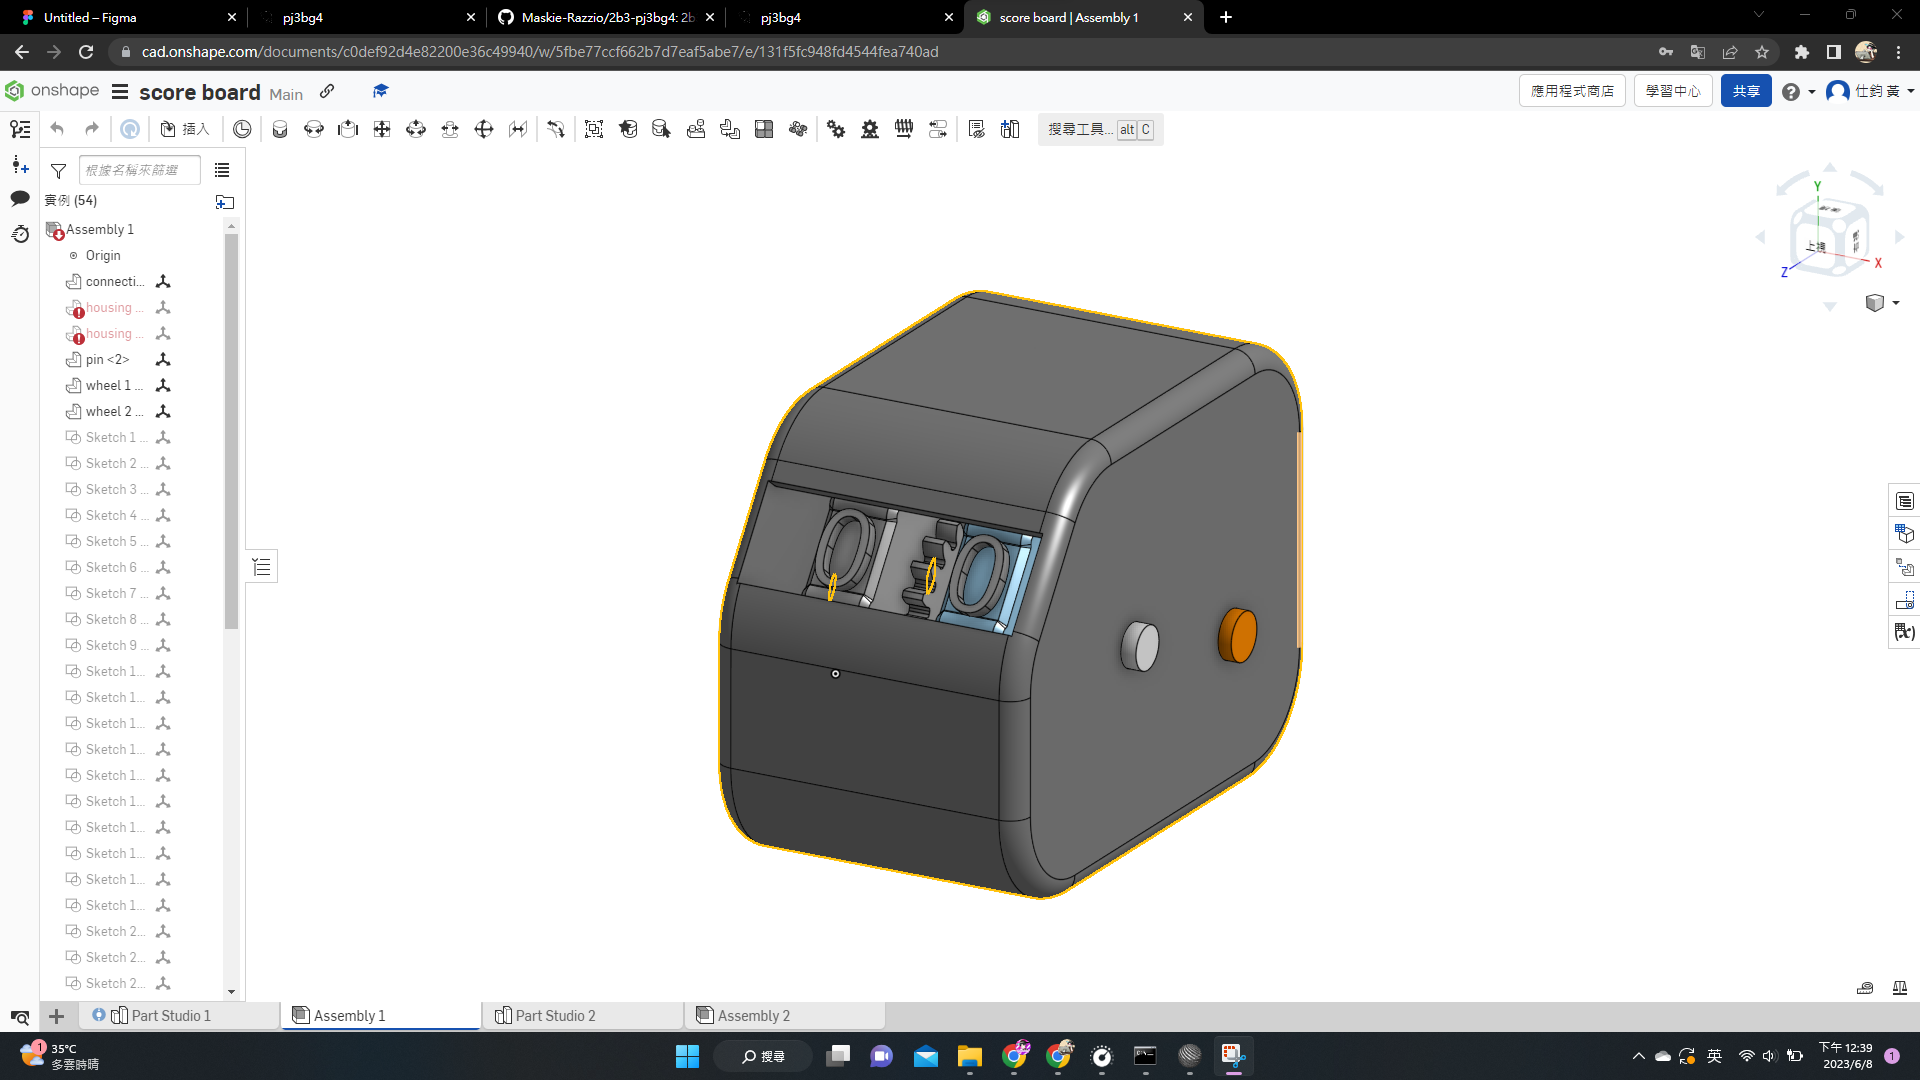
\includegraphics[width=0.3\textwidth]{螢幕擷取畫面 2023-06-08 123921.png}
    \label{fig:image1}
  }
  \hfill
  \subfigure[改良三代記分板-2]{
    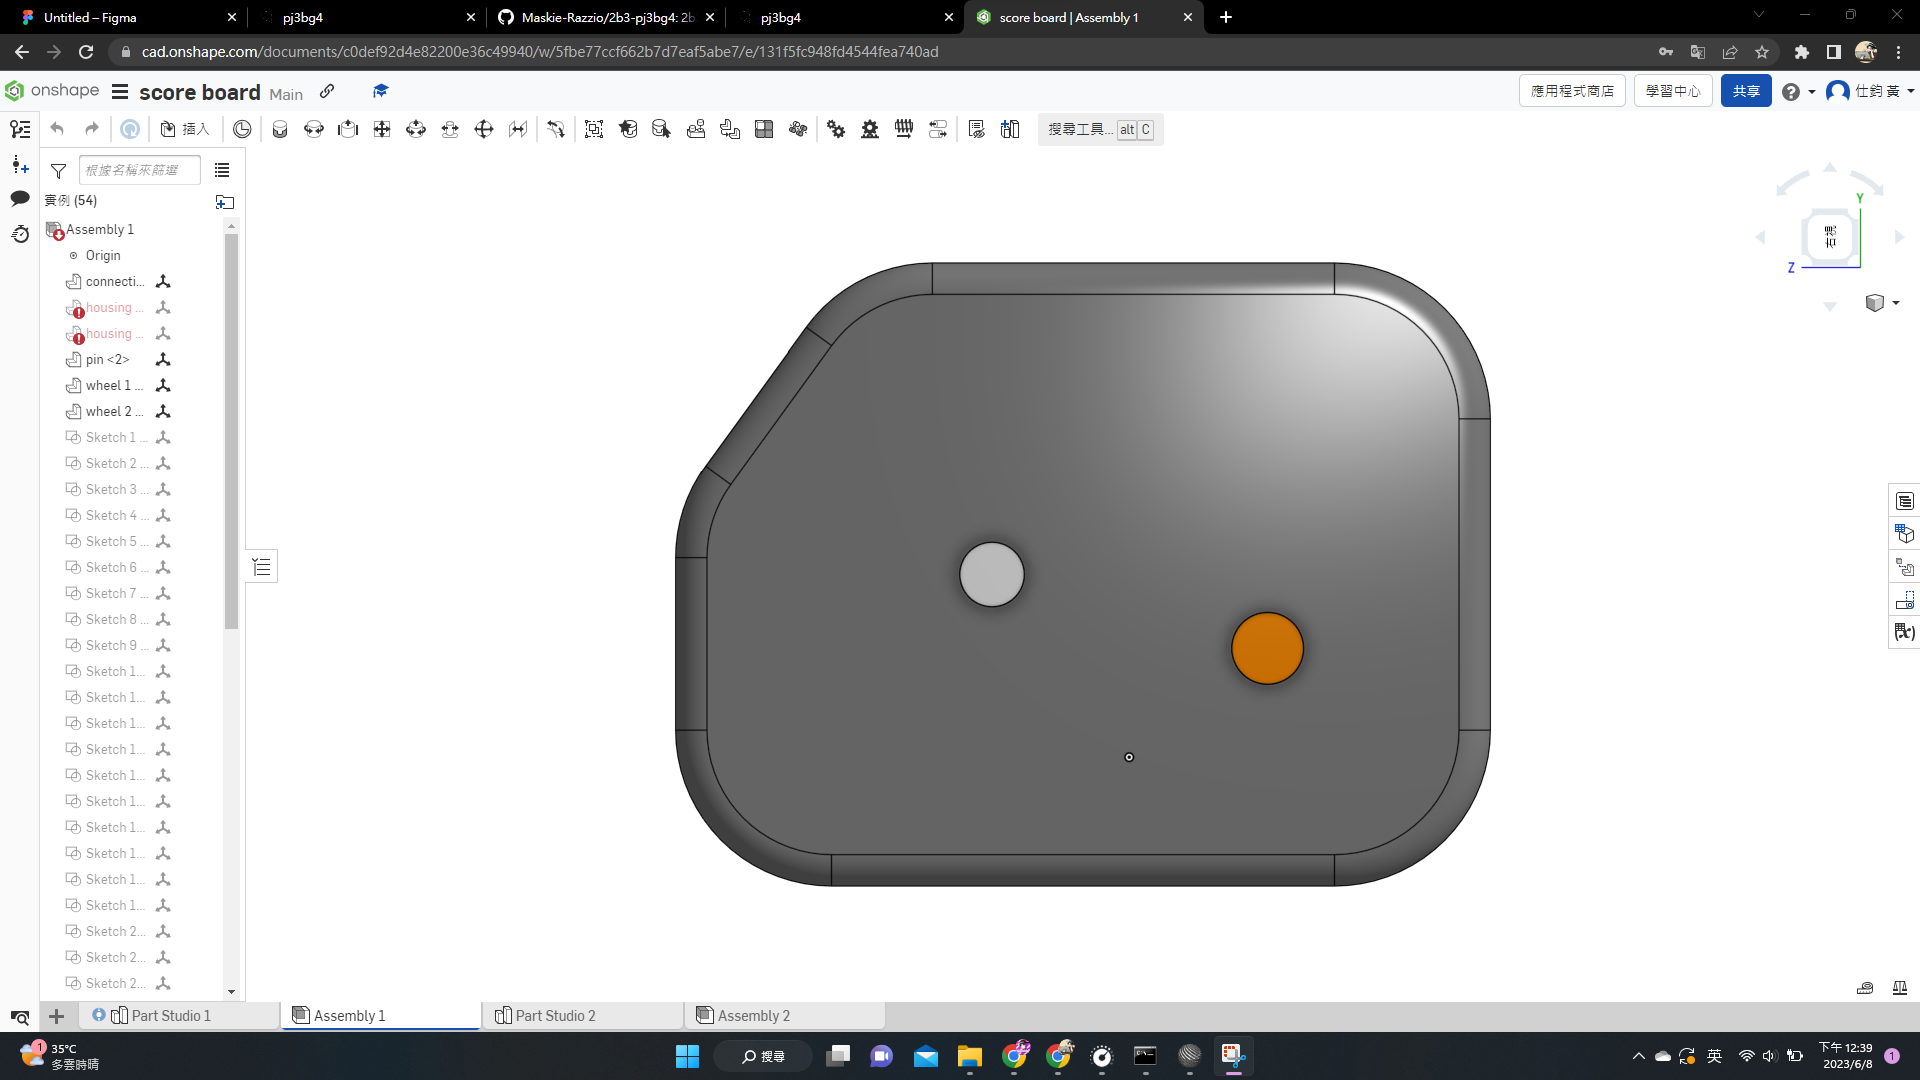
\includegraphics[width=0.3\textwidth]{螢幕擷取畫面 2023-06-08 124004.png}
    \label{fig:image2}
  }
  \hfill
  \subfigure[改良三代記分板-3]{
    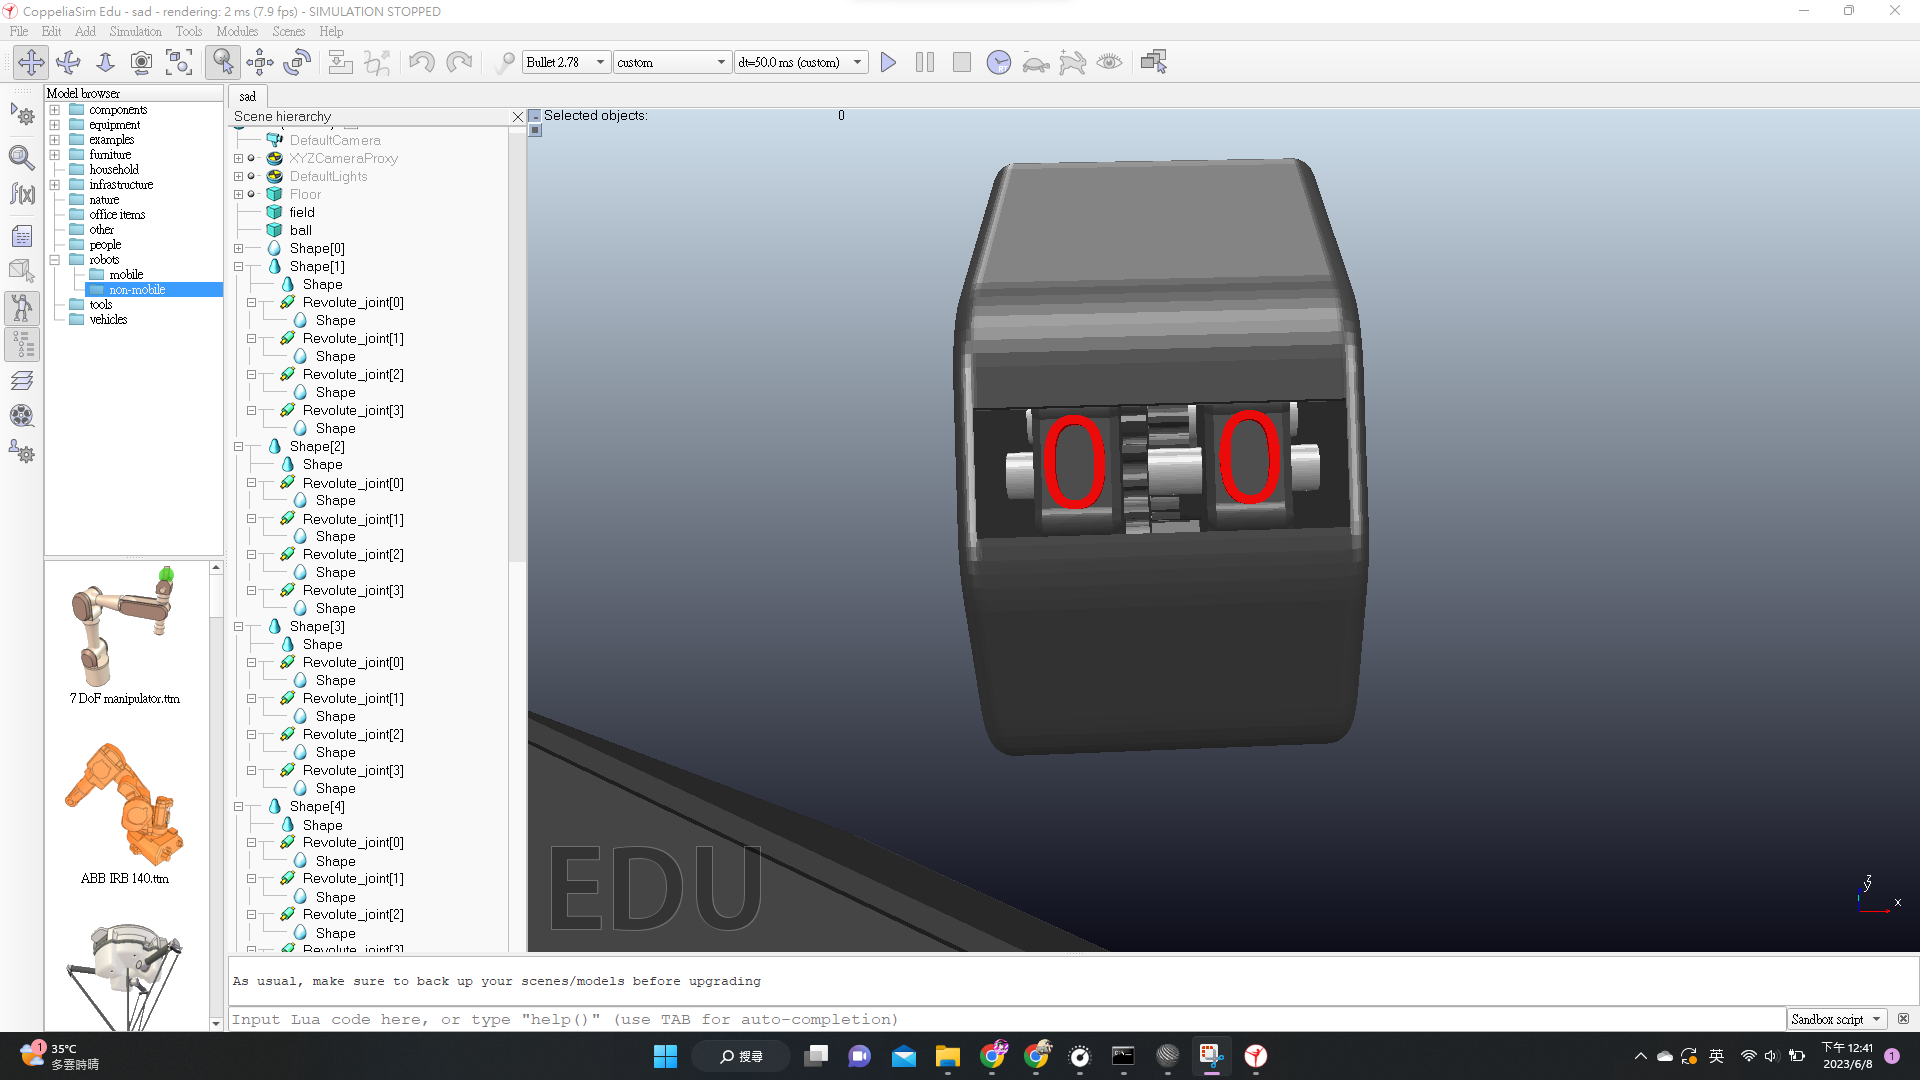
\includegraphics[width=0.3\textwidth]{螢幕擷取畫面 2023-06-08 124125.png}
    \label{fig:image3}
  }
  \hfill

  \caption{改良三代記分板設計圖}
  \label{fig:multi_images}
\end{figure}

\begin{flushleft}
\fontsize{14pt}{20pt}\sectionef\hspace{12pt}\quad 加入以程式控制的倒計時與記名功能。
\end{flushleft}

\begin{figure}[h]
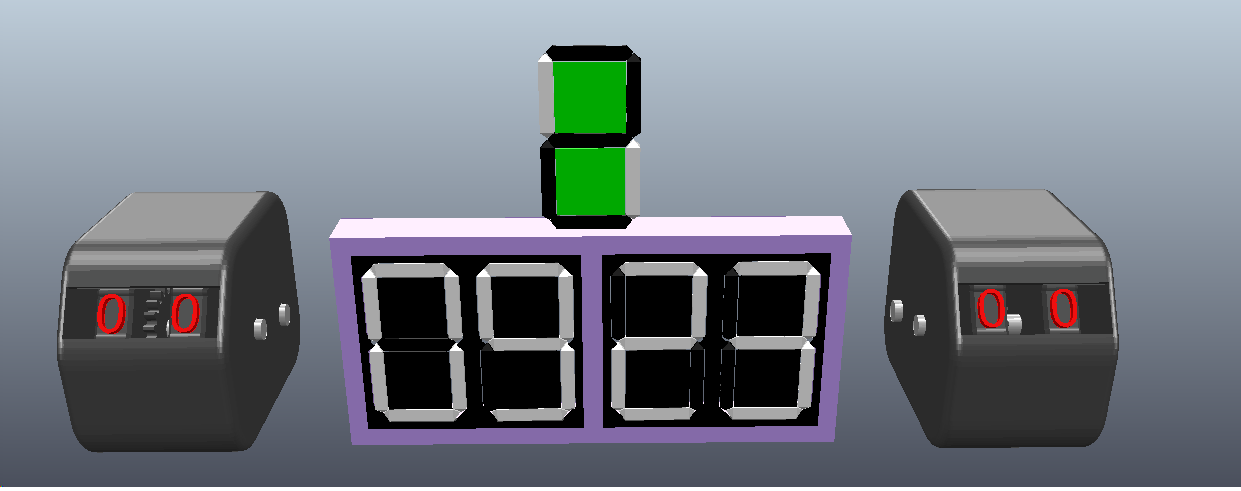
\includegraphics[width=1\textwidth]{615記分板.png}
\caption{最新計分板}
\end{figure}

\newpage
\section{球場}
\begin{flushleft}
\fontsize{14pt}{20pt}\sectionef\hspace{12pt}\quad 初代場景:
\end{flushleft}
\begin{figure}[h]
\includegraphics[width=0.5\textwidth]{CS-field.png}
\caption{初代場景}
\end{figure}

\begin{flushleft}
\fontsize{14pt}{20pt}\sectionef\hspace{12pt}\quad 由於原本的場景會拖累運行速度,故重新製作場景:
\end{flushleft}
\begin{figure}[h]
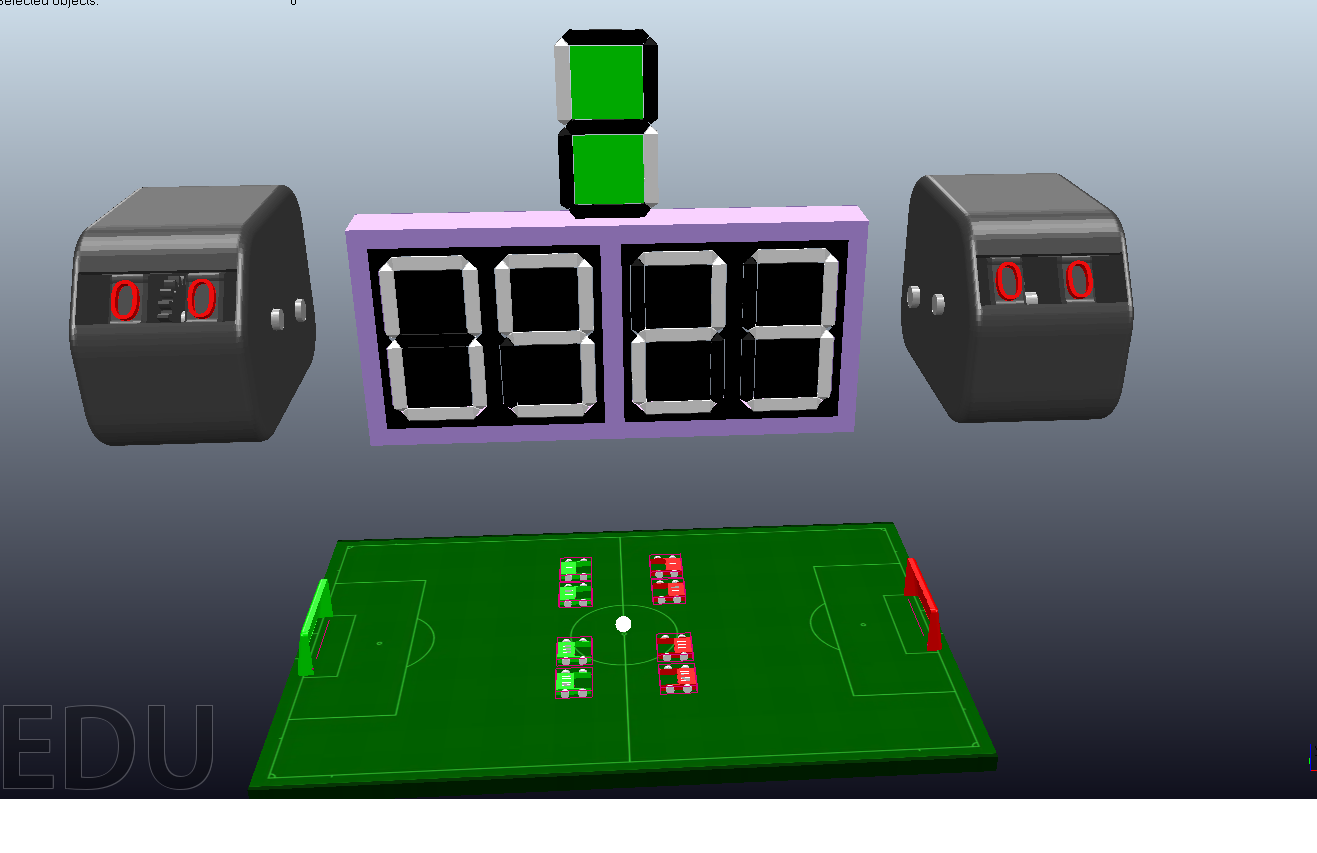
\includegraphics[width=0.5\textwidth]{615場景.png}
\caption{新版本球場}
\end{figure}

\newpage
\section{球員}

\subsection{666系列:}
\begin{figure}[h]
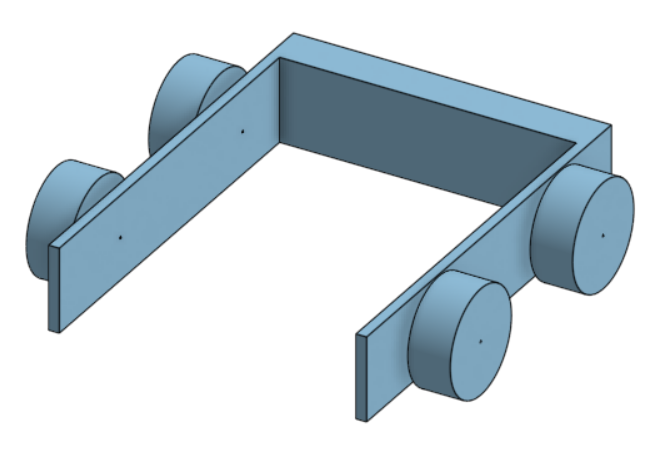
\includegraphics[width=0.5\textwidth]{666.png}
\caption{41023228測試用666}
\end{figure}

\subsection{robot-00系列:}
\begin{figure}[h]
\includegraphics[width=0.5\textwidth]{robot-00系列.png}
\caption{由41023247製作}
\end{figure}

\newpage
\subsection{Maskie Razzio系列:}

\begin{figure}[h]
  \centering
  \subfigure[機器人2:bulldozer6]{
    \includegraphics[width=0.3\textwidth]{bulldozer6.png}
    \label{fig:image1}
  }
  \hfill
  \subfigure[機器人3:bulldozer4]{
    \includegraphics[width=0.3\textwidth]{bulldozer4.png}
    \label{fig:image2}
  }
  \hfill
  \subfigure[機器人4:tank]{
    \includegraphics[width=0.3\textwidth]{tank.png}
    \label{fig:image3}
  }
  \hfill
  \subfigure[機器人5:castle]{
    \includegraphics[width=0.3\textwidth]{castle.png}
    \label{fig:image3}
  }
  \hfill
  \subfigure[機器人6:Eye of Sauron]{
    \includegraphics[width=0.3\textwidth]{eye.png}
    \label{fig:image3}
  }
  \hfill
  \subfigure[機器人7:cat]{
    \includegraphics[width=0.3\textwidth]{cat.png}
    \label{fig:image3}
  }
  \hfill
  \subfigure[機器人8:battlebot]{
    \includegraphics[width=0.3\textwidth]{battlebot.png}
    \label{fig:image3}
  }
  \hfill
  \subfigure[機器人?:wheelchair]{
    \includegraphics[width=0.3\textwidth]{wheelchair.png}
    \label{fig:image3}
  }
  \hfill
  
  \caption{Maskie Razzio系列}
  \label{fig:multi_images}
\end{figure}

\newpage
\subsection{四代與五代球員}

\begin{flushleft}
\fontsize{14pt}{20pt}\sectionef\hspace{12pt}\quad 由於將前幾代球員放入CoppeliaSim裡,會使CoppeliaSim之幀數過高,使其整體運行過慢,因此將機器人重新設計。
\end{flushleft}

\begin{figure}[h]
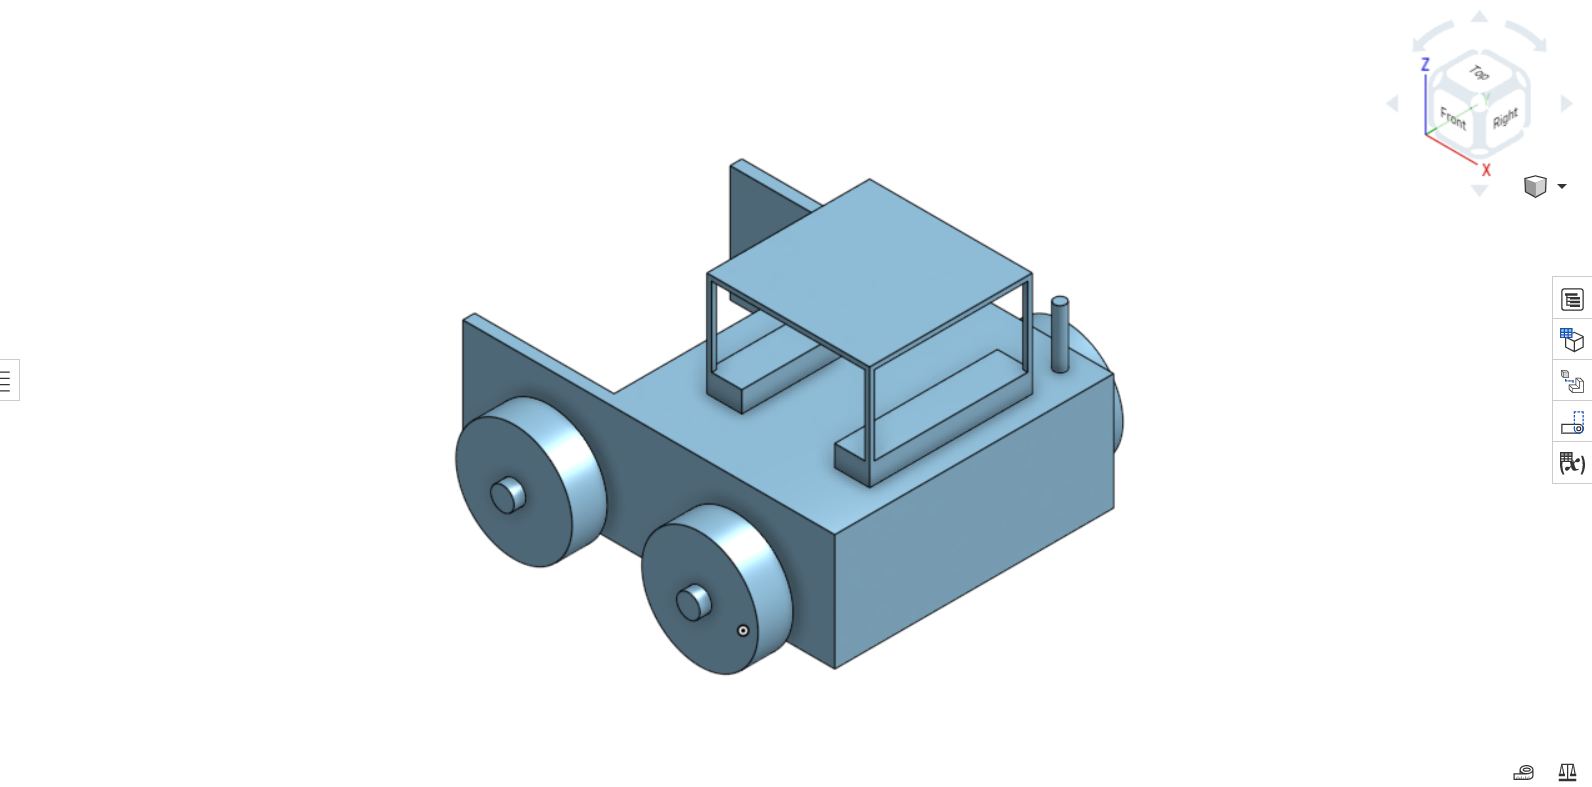
\includegraphics[width=1\textwidth]{robot-cccccc系列.png}
\caption{四代球員:robot-cccccc系列}
\end{figure}

\begin{figure}[h]
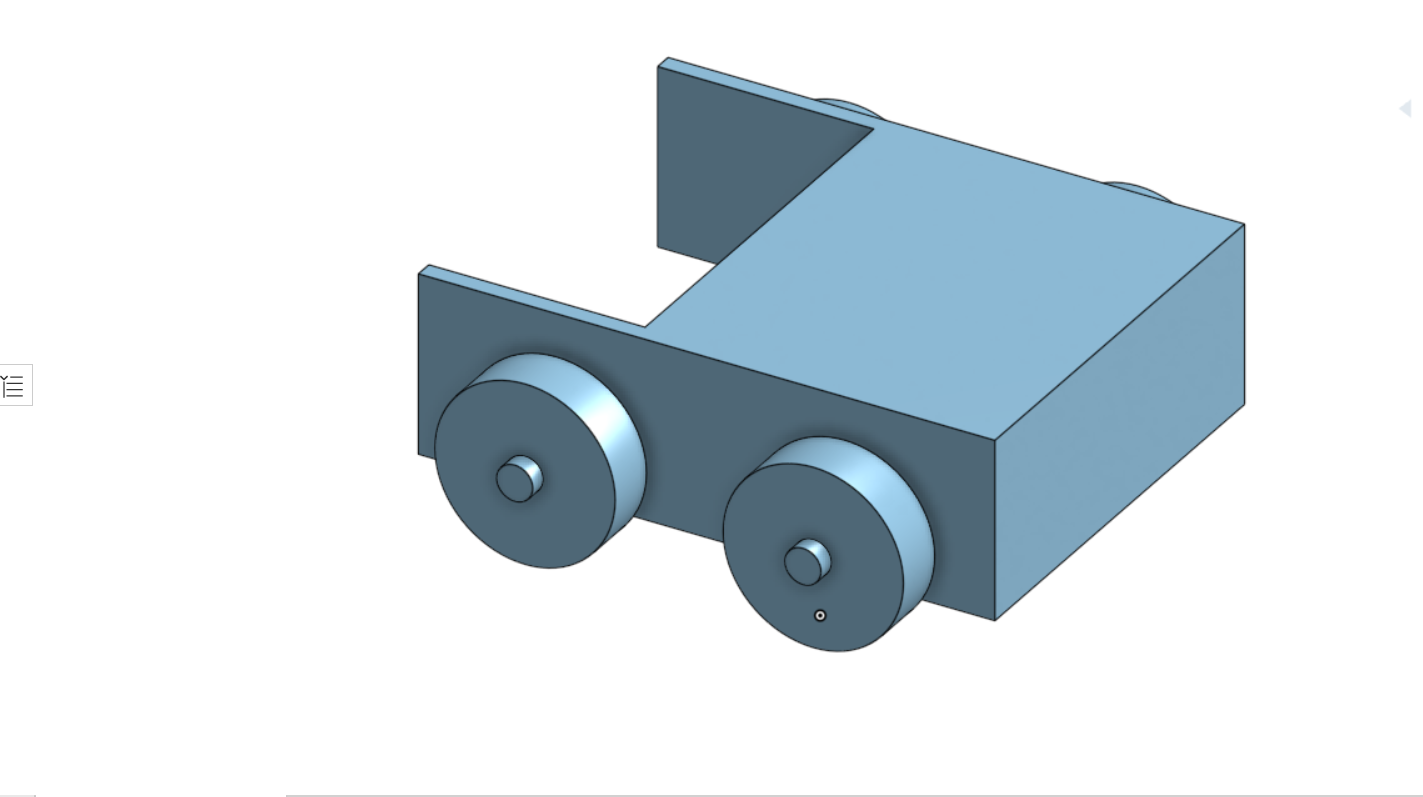
\includegraphics[width=1\textwidth]{robot-110系列.png}
\caption{五代球員:robot-110系列}
\end{figure}